\documentclass[12pt,a4paper]{article}
\usepackage[utf8]{inputenc}
\usepackage[german]{babel}
\usepackage[T1]{fontenc}
\usepackage{amsmath}
\usepackage{amsfonts}
\usepackage{amssymb}
\usepackage{graphicx}
\usepackage{siunitx}
\usepackage[left=2cm,right=2cm,top=2cm,bottom=2cm]{geometry}
\author{Tim}

\begin{document}
\sisetup{separate-uncertainty = true}
	\setlength{\parindent}{0pt} 
	\begin{center}
		{\LARGE Versuchsprotokoll}\\
		\begin{large}
			zum Grundpraktikum Physik Teil II\\[0.4cm]
			an der RWTH Aachen\\
			I. Physikalisches Institut B\\[4.5cm]
			\Large\textbf{\textsl{E-Lehre}}\\[4cm]
			\normalsize\textit{vorgelegt\\von}\\[0.4cm]
			\large{Moritz Berger\\Tim Herbermann\\Gerald Kolter\\Sebastian Siebert}\\[1cm]
			\large \textit{Gruppe A07} \\ [3cm]
			\large \textbf{Sommersemester 2017}
		\end{large}
	\end{center}
	\newpage
	
	\tableofcontents
	\newpage


\section{Grundlagen}

\subsection{Versuchsbeschreibung}
In den folgenden Versuchen wurde die Güte von Serien- und Parallelschwingkreisen auf verschiedene Arten bestimmt. Zusätzlich wurde in einem letzten Aufbau ein Hoch- bzw. Tiefpass untersucht.

\subsection{Physikalische Grundlagen}

\paragraph{Serienkreis}
Aus der Kirchhoffschen Maschenregel ergibt sich eine Differentialgleichung zur Beschreibung der erzwungenen Schwingung.

\begin{equation}
\frac{U}{L} = \frac{d^2 Q}{dt^2}+\frac{R}{L}\frac{dQ}{dt}+\frac{1}{LC} Q
\end{equation}



Dabei ergibt sich der maximale Strom im Kreis bei Resonanz für
\begin{equation}
\omega_0 = \frac{1}{\sqrt{LC}}
\end{equation} 

Die Güte des Schwingkreises ist definiert durch
\begin{equation}
Q_s = \frac{1}{R} \sqrt{\frac{L}{C}}
\label{equ:Guete_Bauteile_Groesse}
\end{equation}

und beschreibt unter anderem den Zusammenhang zwischen angelegter Spannung und Spannungsüberhöhung im Resonanzfall:

\begin{equation}
\frac{U_L(\omega_0)}{U(\omega_0)} = Q_s 
\label{equ:Guete_Spannungsüberhöhung}
\end{equation}

Man stellt fest, dass die Güte sich auch noch als Quotient aus Resonanzfrequenz und Breite der Resonanzkurve bestimmen lässt:
\begin{equation}
\dfrac{\omega_0}{\Delta \omega} = \dfrac{\omega_0}{2d} = \dfrac{\omega_0 L}{R} = \dfrac{1}{R \omega_0 L} = \dfrac{1}{R} \cdot \sqrt{\dfrac{L}{C}} =: Q_S
\label{equ:Guete_Resonanzbreite}
\end{equation}

Man stellt fest, dass die Güte sich auch noch als Quotient aus Resonanzfrequenz und Breite der Resonanzkurve bestimmen lässt:
\begin{equation}
\dfrac{\omega_0}{\Delta \omega} = \dfrac{\omega_0}{2d} = \dfrac{\omega_0 L}{R} = \dfrac{1}{R \omega_0 L} = \dfrac{1}{R} \cdot \sqrt{\dfrac{L}{C}} =: Q_S
\label{equ:Guete_Resonanzbreite}
\end{equation}


\paragraph{Parallelschwingkreis}
Aus der Knotenregel kann ebenfalls eine Differentialgleichung zur Beschreibung des Parallelschwingkreises hergeleitet werden.

Aus dieser kann ebenfalls die Resonanzfrequenz bestimmt werden.

\begin{equation}
\omega_0 = \sqrt{\frac{1-\frac{C}{L}\cdot R_L^2}{LC}}
\end{equation} 

Für große Widerstände im Kreis ergibt sich für die Güte der Schaltung näherungsweise der Zusammenhang:

\begin{equation}
Q_P = \frac{1}{R_L} \sqrt{\frac{L}{C}}
\label{equ:Güte_Bauteile}
\end{equation}

Im Falle des Parallelschwingkreises kommt es bei Resonanz zu einer Stromüberhöhung. Auch hier ergibt sich der Zusammenhang:

\begin{equation}
\frac{(I_L)_0}{I_0} = Q_p
\end{equation}

\paragraph{Hoch -und Tiefpass}
Ein Hoch- bzw. Tiefpass 1. Ordnung besteht aus einer Serienschaltung von Widerstand und Kondensator. Durch Anlegen einer Wechselspannung werden, abhängig davon wo die Spannung abgegriffen wird, entweder große oder kleine Frequenzen blockiert bzw. durchgelassen.

Der Hochpass ergibt sich durch Spannungsabgriff am Widerstand. Die Übertragsfunktion ergibt sich dabei zu:

\begin{equation}
\frac{U_a}{U_e} = \frac{1}{\sqrt{(\frac{1}{\omega C R})^2+1}}
\end{equation}

Den Tiefpass erhält man dann entsprechend durch Abgriff am Kondensator. Die Übertragsfunktion lautet:

\begin{equation}
\frac{U_a}{U_e} = \frac{1}{\sqrt{1+(\omega C R)^2}}
\end{equation}

\section{Serienschwingkreis}

\subsection{Aufbau und Durchführung}


\subsection{Aufbau und Durchführung}

\begin{figure}
\centering
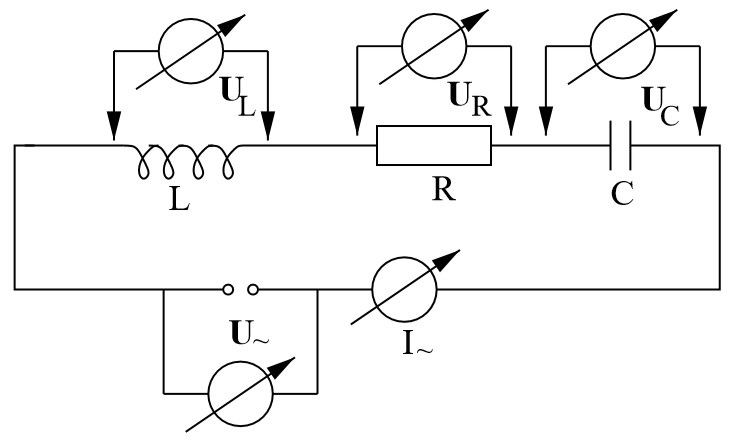
\includegraphics[scale=0.8]{Bilder/AufbauSerie.png}
\caption{Schaltbild zum Serienschwingkreis. Die Spannungsmessung am Ohmschen Widerstand wurde nur im Rahmen der Vorauswertung mit dem Oszilloskop durchgeführt.}
\label{fig:AufbauSerie}
\end{figure}

Der wesentliche Versuchsaufbau ist in Abbildung \ref{fig:AufbauSerie} gezeigt. Für alle Versuche zum Serienkreis wurde der Kondensator mit Nominalkapazität $C=\SI{4,7}{\micro \F}$ und die Spule mit 250 Windungen verwendet.

Die Messung der Spannung am Ohmschen Widerstand findet dabei nur im Rahmen des Vorversuches mit einem Oszilloskop statt.
Im Hauptversuch werden Gesamtspannung und Strom über das Power-CASSY, welches gleichzeitig als Spannungsquelle fungiert, als Effektivwerte gemessen. Die abfallenden Spannungen an Spule und Kondensator werden mit dem Sensor-CASSY ebenfalls als Effektivwerte aufgezeichnet. Der Messvorgang wird mit verschiedenen Widerständen wiederholt.

Die am Power-CASSY eingestellte Wechselspannungsamplitude wurde abhängig vom Widerstand gewählt. Der Gleichspannungsoffset beträgt $U = \SI{0}{V}$. Die Signalform ist eine Sinusschwingung.

Die Frequenz wurde automatisch über die Formel $f_1 = f_0 +(n-1) \cdot \Delta f$ automatisch variiert. Über eine die Zusatzbedingung der Form$f_1 < f_{Grenz} and delta t > 2$ wurde ein Abbruch bei einer maximalen Frequenz sowie das Aufzeichnen des Messwertes nach dem Einschwingvorgang gewährleistet. Der Messbereich der Spannung ist 0-7V. Start- und Endfrequenz wurden dabei für jeden Widerstand unterschiedlich gewählt.

\subsection{Vorauswertung: Oszilloskop}
Im Rahmen der Vorauswertung wurde die Spannung am Ohmschen Widerstand und die gesamte abfallende Spannung mittels Oszilloskop gemessen. Für Gruppe B wurde der Widerstand mit Nominalwert $R = 5,1 \Omega$ verwendet. Die Frequenz der angelegten Wechselspannung wird über den Frequenzgenerator eingestellt.\\

Zur Bestimmung der Resonanzfrequenz werden die gemessenen Spannungen an beiden Kanälen im Oszilloskop gegeneinander aufgetragen. Die Frequenz wurde so eingestellt, dass die Ellipse verschwindet und die Spannungswerte eine Gerade bilden. Der entsprechende Frequenzwert ist die Resonanzfrequenz
Zur Bestimmung der Resonanzbreite werden in der Zeitdarstellung des Oszilloskops diejenigen Frequenzen bestimmt, für die die Amplitude der Spannung am Widerstand um den Faktor $\sqrt{2}$ kleiner als im Resonanzfall ist. 

Es gilt

\begin{equation}
\Delta f = f_2 - f_1 \quad \Rightarrow \quad Q = \frac{f_0}{\Delta f}
\end{equation}

und mittels Fehlerfortpflanzung:

\begin{equation}
\sigma_{\Delta f} = \sqrt{\sigma_{f_1}^2+\sigma_{f_2}^2} \qquad \sigma_Q = Q \sqrt{(\frac{\sigma_{f_0}}{f_0})^2 + (\frac{\sigma_{\Delta f}}{\Delta f})^2}
\end{equation}

Die Ergebnisse der Voruntersuchung sind für beide Gruppen in Tabelle \ref{tab:Voruntersuchung} dargestellt.

\begin{table}
\centering
\begin{tabular}{|c|c|c|c|c|}
\hline
Gruppe & $f$/Hz & $f_1$/Hz & $f_2$/Hz & Q\\
\hline
A & & & &\\
\hline
B & $2149 \pm 2$ & $1755 \pm 4$ & $2614 \pm 4$ & $2,50 \pm 0,02$\\
\hline
\end{tabular}
\caption{Ergebnisse der Voruntersuchung mittels Oszilloskop}
\label{tab:Voruntersuchung}
\end{table}


Eine zweite Voruntersuchung durch Bestimmen der Spannungsüberhöhung im Resonanzfall war aus Zeitgründen nicht möglich.

\subsection{Auswertung}
Zur Bestimmung der Güte eines Serienschwingkreises gibt es die folgenden 4 Möglichkeiten:
\begin{enumerate}
\item Man misst die Resonanzfrequenz und die Breite der Resonanzkurve. Die Güte ist dann gemäß Gl. \ref{equ:Guete_Resonanzbreite} der Quotient aus beiden.
\item Ein analoges Verfahren lässt sich mit der Phasenverschiebung durchführen: Die Resonanzfrequenz ist dann bei $\varphi = 0$ und die Breite $\Delta \omega$ ist zwischen $\varphi = \pm \ang{45}$.
\item Gemäß Gl. \ref{equ:Guete_Spannungsüberhöhung} lässt sich die Güte auch aus der Spannungsüberhöhung an der Resonanzfrequenz bestimmen.
\item Mit Gl. \ref{equ:Guete_Bauteile} kann die Güte aus den Größen der Bauteilen berechnet werden.
\end{enumerate}

\subsubsection{Gruppe A}
Für die Auswertungsmöglichkeiten 1-3 wurden die jeweiligen Werte jeweils abgelesen und automatisiert berechnet.\\
Die automatisiert berechneten Werte gehen über die einzelnen Messpunkte. Dabei werden Schnittpunkte immer als der Mittelwert der beiden Messpunkte, zwischen denen der Schnittpunkt liegt, approximiert. Für die Bestimmung des Fehlers auf diese Berechnung wird eine Gleichverteilung angenommen.\\

\paragraph{1. Resonanzfrequenz und Breite der Resonanzkurve}\mbox{}\\
\begin{figure}
\centering
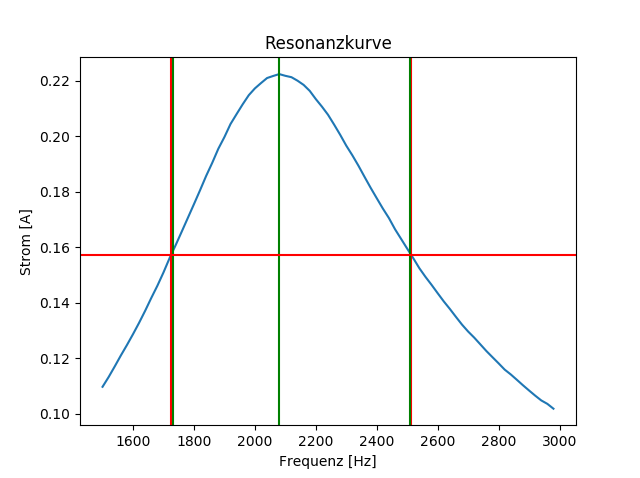
\includegraphics[scale=0.8]{Bilder/Serie_Resonanzkurve_A_5.png}
\caption{Resonanzkurve des Aufbaus mit dem $\SI{5}{\ohm}$ Widerstand. Die waagerechte Linie markiert die Stelle bei der $I = \frac{I_{max}}{\sqrt{2}}$ gilt. Die senkrechten Linien sind die Auswertungslinien (rot = abgelesen, grün = automatisiert ausgerechnet).}
\label{fig:Serie_Resonanzkurve_A_5}
\end{figure}
\begin{figure}
\centering
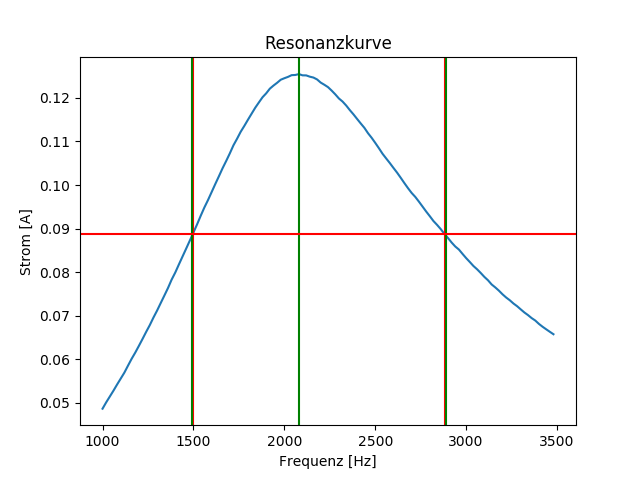
\includegraphics[scale=0.8]{Bilder/Serie_Resonanzkurve_A_10.png}
\caption{Resonanzkurve des Aufbaus mit dem $\SI{10}{\ohm}$ Widerstand. Die waagerechte Linie markiert die Stelle bei der $I = \frac{I_{max}}{\sqrt{2}}$ gilt. Die senkrechten Linien sind die Auswertungslinien (rot = abgelesen, grün = automatisiert ausgerechnet).}
\label{fig:Serie_Resonanzkurve_A_10}
\end{figure}
Abbildung \ref{fig:Serie_Resonanzkurve_A_5} zeigt die Resonanzkurve für den Aufbau mit dem $\SI{5}{\ohm}$ Widerstand. \\
Abbildung \ref{fig:Serie_Resonanzkurve_A_10} zeigt die Resonanzkurve für den Aufbau mit dem $\SI{10}{\ohm}$ Widerstand.

\begin{table}
\centering
\begin{tabular}{|c|c|c|c||c|c|c|}
\hline
Widerstand & $f_0$/Hz & $f_1$/Hz & $f_2$/Hz & $f_0$/Hz & $f_1$/Hz & $f_2$/Hz \\
\hline
$\SI{5}{\ohm}$ & 2080 & 1724.925 & 2513.051 & 2080 & 1730 & 2510 \\
\hline
$\SI{10}{\ohm}$ & 2080 & 1495.616 & 2882.037 & 2080 & 1490 & 2890 \\
\hline
\end{tabular}
\caption{Auswertungswerte der Resonanzkurve mit dem Strom im Serienschwingkreis von Gruppe A. Links sind die abgelesenen Werte, rechts die automatisiert berechneten.}
\label{tab:StromResonanz_A}
\end{table}

Tabelle \ref{tab:StromResonanz_A} zeigt die abgelesenen und automatisiert berechneten Werte für die Resonanzfrequenz und die beiden die Resonanzbreite begrenzenden Frequenzen. Auffällig ist, dass die Resonanzfrequenz beim Ablesen und bei der automatisierten Auswertung identisch ist. Dies liegt daran, dass die Resonanzkurve durch die geringe Punktdichte eine klare Spitze aufweist, weil es einen größten Messpunkt gibt. Daher ist der abgelesene Wert zwangsweise identisch mit dem Maximum.

Die Unsicherheit bei der automatisierten Rechnung wird mit dem Abstand zweier Messpunkte bei Annahme einer Gleichverteilung angegeben:
\begin{equation*}
\sigma_{f_{berechnet}} = \dfrac{\SI{20}{Hz}}{\sqrt{12}}
\end{equation*}

Die Unsicherheit beim Ablesen wird mit 
\begin{equation*}
\sigma_{f_{berechnet}} = \SI{5}{Hz}
\end{equation*}
angenommen.\\
Die Fehlerfortpflanzung ist für die Auswertung durch Ablesen und die automatisierte Auswertung identisch:\\
Nach Gl. \ref{equ:Guete_Resonanzbreite} pflanzt sich der Fehler auf die Frequenz fort:
\begin{equation}
\dfrac{\sigma_Q}{Q} = \sqrt{\left( \dfrac{\sigma_f}{f_0} \right)^2 + \left( \dfrac{\sigma_{\Delta f}}{\Delta f} \right)^2} = \sqrt{\left( \dfrac{\sigma_f}{f_0} \right)^2 + \left( \dfrac{\sqrt{2} \cdot \sigma _f}{\Delta f} \right)^2}
\label{equ:FehlerGuete_FehlerFrequenz}
\end{equation}

Damit ergibt sich aus dieser Methode die Güte des Schwingkreises mit dem $\SI{5}{\ohm}$ Widerstand mit Gl. \ref{equ:Guete_Resonanzbreite} und Gl. \ref{equ:FehlerGuete_FehlerFrequenz} zu:
\begin{equation*}
Q_{abgelesen} = \num{2.6392(245)} \qquad Q_{berechnet} = \num{2.6667(289)}
\end{equation*}
Und für den $\SI{10}{\ohm}$ Widerstand:
\begin{equation*}
Q_{abgelesen} = \num{1.5003(85)} \qquad Q_{berechnet} = \num{1.4857(96)}
\end{equation*}

\paragraph{2. Phasenverschiebung}\mbox{}\\
\begin{figure}
\centering
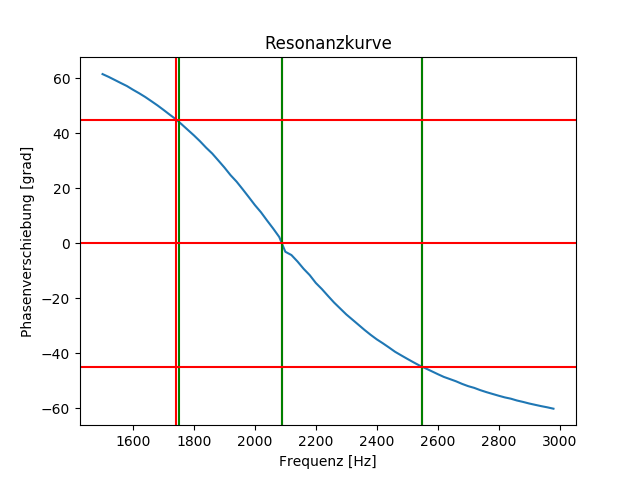
\includegraphics[scale=0.8]{Bilder/Serie_Phasenverschiebung_A_5.png}
\caption{Phasenverschiebung des Aufbaus mit dem $\SI{5}{\ohm}$ Widerstand. Die waagerechten Linien markieren die Stellen bei der $\varphi = 0, \pm \ang{45}$. Die senkrechten Linien sind die Auswertungslinien (rot = abgelesen, grün = automatisiert ausgerechnet).}
\label{fig:Serie_Phasenverschiebung_A_5}
\end{figure}
\begin{figure}
\centering
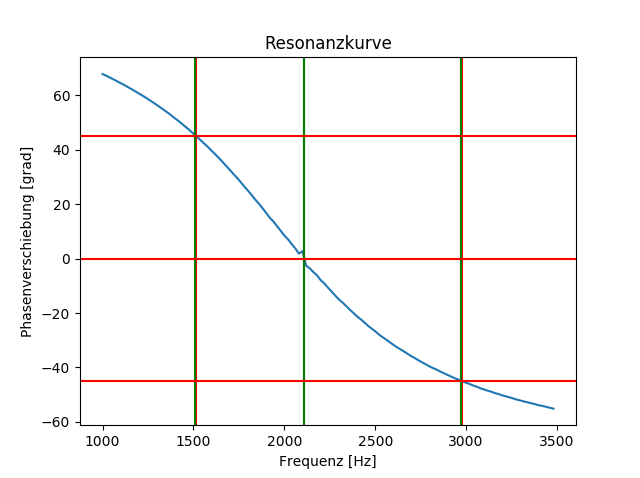
\includegraphics[scale=0.8]{Bilder/Serie_Phasenverschiebung_A_10.png}
\caption{Phasenverschiebung des Aufbaus mit dem $\SI{10}{\ohm}$ Widerstand. Die waagerechten Linien markieren die Stellen bei der $\varphi = 0, \pm \ang{45}$ ist. Die senkrechten Linien sind die Auswertungslinien (rot = abgelesen, grün = automatisiert ausgerechnet).}
\label{fig:Serie_Phasenverschiebung_A_10}
\end{figure}
Abbildung \ref{fig:Serie_Phasenverschiebung_A_5} zeigt die Phasenverschiebung für den Aufbau mit dem $\SI{5}{\ohm}$ Widerstand. \\
Abbildung \ref{fig:Serie_Phasenverschiebung_A_10} zeigt die Phasenverschiebung für den Aufbau mit dem $\SI{10}{\ohm}$ Widerstand.

\begin{table}
\centering
\begin{tabular}{|c|c|c|c||c|c|c|}
\hline
Widerstand & $f_0$/Hz & $f_1$/Hz & $f_2$/Hz & $f_0$/Hz & $f_1$/Hz & $f_2$/Hz \\
\hline
$\SI{5}{\ohm}$ & 2088.437 & 1742.037 & 2549.634 & 2090 & 1750 & 2550 \\
\hline
$\SI{10}{\ohm}$ & 2110.274 & 1516.288 & 2975.858 & 2110 & 1510 & 2970 \\
\hline
\end{tabular}
\caption{Auswertungswerte der Phasenverschiebung im Serienschwingkreis von Gruppe A. Links sind die abgelesenen Werte, rechts die automatisiert berechneten.}
\label{tab:StromPhasenverschiebung_A}
\end{table}

Tabelle \ref{tab:StromPhasenverschiebung_A} zeigt die abgelesenen und automatisiert berechneten Werte für die Resonanzfrequenz und die beiden die Resonanzbreite begrenzende Frequenzen. \\
Die automatisierte Auswertung wurde genauso realisiert wie bei Methode 1. \\
Die Fehlerrechnung kann komplett aus der Auswertung nach der ersten Methode übernommen werden (siehe Gl. \ref{equ:FehlerGuete_FehlerFrequenz}). \\
Damit ergibt sich aus dieser Methode die Güte des Schwingkreises mit dem $\SI{5}{\ohm}$ Widerstand mit Gl. \ref{equ:Guete_Resonanzbreite} und Gl. \ref{equ:FehlerGuete_FehlerFrequenz} zu:
\begin{equation*}
Q_{abgelesen} = \num{2.5860(235)} \qquad Q_{berechnet} = \num{2.6125(276)}
\end{equation*}
Und für den $\SI{10}{\ohm}$ Widerstand:
\begin{equation*}
Q_{abgelesen} = \num{1.4458(78)} \qquad Q_{berechnet} = \num{1.4452(90)}
\end{equation*}

\paragraph{3. Spannungsüberhöhung}\mbox{}\\
\begin{figure}
\centering
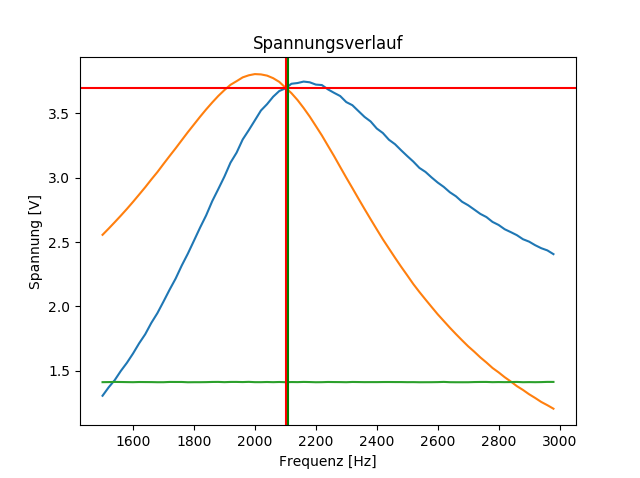
\includegraphics[scale=0.8]{Bilder/Serie_Spannungsueberhoehung_A_5.png}
\caption{Verlauf der Kondensator- (orange), Spulen- (blau) und angelegten Spannung (grün) beim Aufbau mit dem $\SI{5}{\ohm}$ Widerstand. Die waagerechte Linie markiert den Spannungswert des Schnittpunktes und die senkrechten Linien die zugehörige Frequenz (rot = abgelesen, grün = automatisiert ausgerechnet).}
\label{fig:Serie_Spannungsueberhoehung_A_5}
\end{figure}
\begin{figure}
\centering
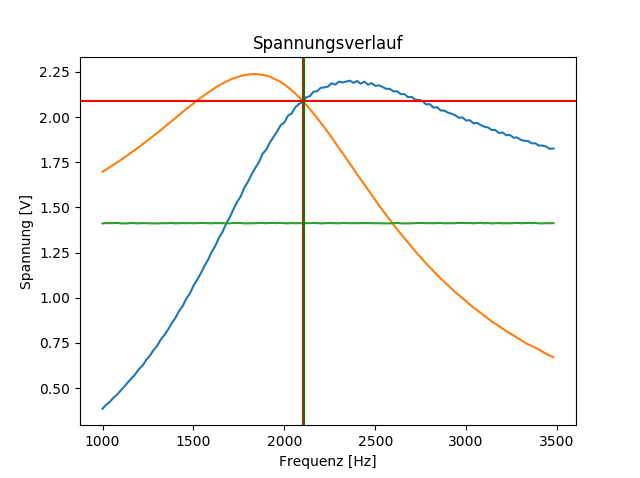
\includegraphics[scale=0.8]{Bilder/Serie_Spannungsueberhoehung_A_10.png}
\caption{Verlauf der Kondensator- (orange), Spulen- (blau) und angelegten Spannung (grün) beim Aufbau mit dem $\SI{10}{\ohm}$ Widerstand. Die waagerechte Linie markiert den Spannungswert des Schnittpunktes und die senkrechten Linien die zugehörige Frequenz (rot = abgelesen, grün = automatisiert ausgerechnet).}
\label{fig:Serie_Spannungsueberhoehung_A_10}
\end{figure}

\begin{table}
\centering
\begin{tabular}{|c|c|c|c||c|c|c|}
\hline
Widerstand & $f_0$/Hz & $U_{L, f_0}$/V & $U_{an, f_0}$/V & $f_0$/Hz & $U_{L, f_0}$/V & $U_{an, f_0}$/V \\
\hline
$\SI{5}{\ohm}$ & 2101.633 & 3.696443 & 1.41231 & 2110 & 3.711449 & 1.412179 \\
\hline
$\SI{10}{\ohm}$ & 2102.349 & 2.086694 & 1.41231 & 2110 & 2.096682 & 1.412179 \\
\hline
\end{tabular}
\caption{Auswertungswerte der Spannungsüberhöhung im Serienschwingkreis von Gruppe A. Links sind die abgelesenen Werte, rechts die automatisiert berechneten.}
\label{tab:Spannungsueberhoehung_A}
\end{table}

Abbildung \ref{fig:Serie_Spannungsueberhoehung_A_5} zeigt die Verläufe von Kondensator-, Spulen- und angelegter Spannung für den Aufbau mit dem $\SI{5}{\ohm}$ Widerstand.\\
Abbildung \ref{fig:Serie_Spannungsueberhoehung_A_10} zeigt die Verläufe von Kondensator-, Spulen- und angelegter Spannung für den Aufbau mit dem $\SI{10}{\ohm}$ Widerstand.\\ 
Tabelle \ref{tab:Spannungsueberhoehung_A} zeigt die abgelesenen und automatisiert berechneten Werte.\\
Als Fehler auf die Spannung wird die Standardabweichung aus der Rauschmessung verwendet:
\begin{equation*}
\sigma _U = \sigma _{U_L} = \sigma _{U_{an}} = \SI{0.0014}{V}
\end{equation*}
Gemäß Gl. \ref{equ:Guete_Spannungsüberhöhung} lässt sich die Fortpflanzung des Fehlers auf die Spannung wie folgt bestimmen:
\begin{equation}
\dfrac{\sigma _Q}{Q} = \sqrt{\left( \dfrac{\sigma _U}{U_{L, f_0}} \right)^2 + \left( \dfrac{\sigma _U}{U_{an, f_0}} \right)^2}
\end{equation}

Damit ergibt sich aus dieser Methode die Güte des Schwingkreises mit dem $\SI{5}{\ohm}$ Widerstand mit Gl. \ref{equ:Guete_Resonanzbreite} und Gl. \ref{equ:FehlerGuete_FehlerFrequenz} zu:
\begin{equation*}
Q_{abgelesen} = \num{2.6170(30)} \qquad Q_{berechnet} = \num{2.6282(28)}
\end{equation*}
Und für den $\SI{10}{\ohm}$ Widerstand:
\begin{equation*}
Q_{abgelesen} = \num{1.4780(20)} \qquad Q_{berechnet} = \num{1.4847(18)}
\end{equation*}

\paragraph{4. Berechnung aus Bauteilen}\mbox{}\\
\begin{table}
\begin{center}
\begin{tabular}{|c|c|}
\hline 
Bauteil & Größe \\ 
\hline 
Spule & \SI{1.2750(3)}{mH} \\ 
\hline 
Kondensator & \SI{4.5975(3)}{\mu F} \\ 
\hline 
\SI{5}{\ohm} Widerstand & \SI{5.1820(3)}{\ohm} \\ 
\hline 
\SI{10}{\ohm} Widerstand & \SI{99.080(3)}{\ohm} \\ 
\hline 
\end{tabular} 
\caption{Größen der für den Aufbau des Serienschwingkreises von Gruppe A verwendeten Bauteile.}
\label{tab:BauteileGroesse_A}
\end{center}
\end{table}

Die charakteristischen Größen der Bauteile wurde mit der Brücke gemessen. Das Ergebnis dieser Messung ist in Tabelle \ref{tab:BauteileGroesse_A} aufgeführt.\\
Die Güte berechnet sich wie Gl. \ref{equ:Guete_Bauteile_Groesse}. Anhand dieser lassen sich auch direkt die Fehler fortpflanzen:
\begin{equation}
\dfrac{\sigma _Q}{Q} = \sqrt{\left( \dfrac{\sigma _R}{R} \right)^2 + \left( \dfrac{\sigma _L}{2 \cdot L} \right)^2 + \left( \dfrac{\sigma _C}{2 \cdot C} \right)^2}
\label{equ:FehlerGuete_FehlerBauteile}
\end{equation}

Damit ergibt sich aus den Bauteilen die Güte des Schwingkreises mit dem $\SI{5}{\ohm}$ Widerstand mit Gl. \ref{equ:Guete_Bauteile_Groesse} und Gl. \ref{equ:FehlerGuete_FehlerBauteile} zu:
\begin{equation*}
Q_{Bauteile} = \num{3.2135(4)}
\end{equation*}
Und für den $\SI{10}{\ohm}$ Widerstand:
\begin{equation*}
Q_{Bauteile} = \num{1.6594(2)}
\end{equation*}


\newpage
\section{Parallelschwingkreis}

\subsection{Auswertung}
\paragraph{1. Resonanzfrequenz und Breite der Resonanzkurve}\mbox{}\\
\begin{figure}
\centering
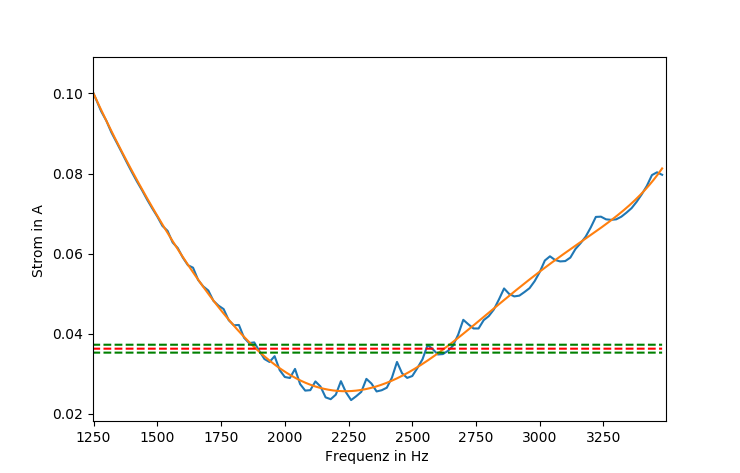
\includegraphics[scale=0.4]{Bilder/Parallel_Iges.png}
\caption{TBD}
\label{fig:Serie_Resonanzkurve_A_5}
\end{figure}

\begin{table}
\begin{tabular}{|c|c|c|c|}
\hline
Messung & 1&2&3\\
\hline
$f_0$ & $2216\pm 50 $ & $2216\pm 65 $ & $2235\pm 80$\\
\hline
$\Delta f$ & $737\pm 64 $ & $488\pm 110 $ & $738\pm 49$\\
\hline
$Q$ & $3.01\pm 0.27 $ & $4.54\pm 1.03 $ & $3.03\pm 0.23$\\
\hline
\end{tabular}
\end{table}


\section{Hoch- und Tiefpass}


In diesem Versuch soll die Übertragsfunktion von Hoch- bzw. Tiefpass aufgezeichnet werden und die charakteristische Frequenz $\omega_0$ des Aufbaus bestimmt werden.

\subsection{Auf und Durchführung}

\begin{figure}
\centering
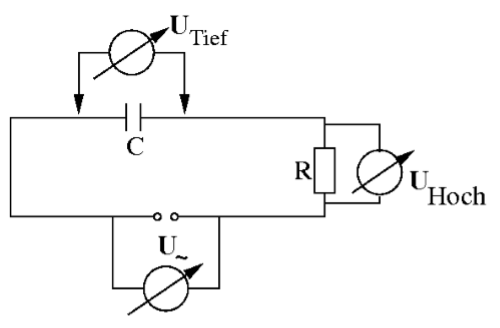
\includegraphics[scale=1.0]{Bilder/AufbauHochTief.png}
\caption{Schaltskizze zum Hoch- bzw Tiefpass. (Quelle: Praktikumsskript S. 94)}
\label{fig:AufbauHochTief}
\end{figure}

Der Versuchsaufbau erfolgt nach der Schaltskizze in Abbildung \ref{fig:AufbauHochTief}. Die Spannungen an Widerstand und Kondensator
werden mit dem Sensor-CASSY aufgezeichnet. Die Spannungsquelle ist erneut durch das Power-CASSY gegeben, welches gleichzeitig die angelegte Spannung misst. Alle Messwerte werden als Effektivwerte gemessen.

Die Frequenz wird wieder automatisch schrittweise bis zu einem maximalen Wert erhöht. Die Einstellungen diesbezüglich sind identisch zu den vorherigen Versuchen. Die Wechselspannungsamplitude wurde zu 5V eingestellt.

Gruppe A verwendet in ihrem Aufbau den $\SI{4,7}{\micro \F}$ Kondensator und den $\SI{100}{\ohm}$ Widerstand. Gruppe B hat einen Kondensator mit gleichem Nominalwert und einen $\SI{10}{\ohm}$ Widerstand benutzt.

\subsection{Auswertung}

\begin{figure}
\centering
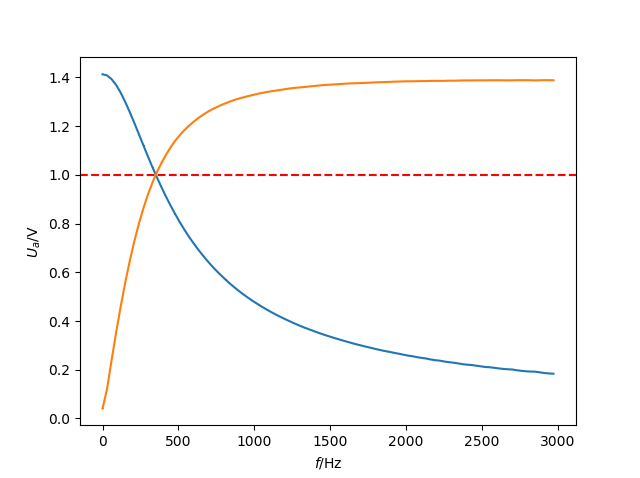
\includegraphics[scale=1.0]{Bilder/RohdatenHochTief_A.png}
\caption{Rohdaten für Gruppe A. eine Hilfslinie bei $\frac{U_{eff}}{\sqrt{2}}$, wobei $U_{eff}$ der Effektivwert der angelegten Spannung ist, eingezeichnet.}
\label{fig:RohdatenHochTief_A}
\end{figure}

\begin{figure}
\centering
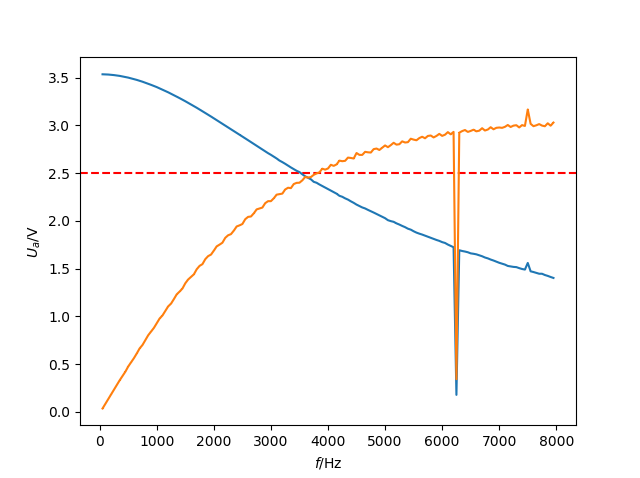
\includegraphics[scale=1.0]{Bilder/RohdatenHochTief_B.png}
\caption{Rohdaten der aufgezeichneten Spannungen für Gruppe B. Es sind Hilfslinien bei $U_{eff}$ und $\frac{U_{eff}}{\sqrt{2}}$, wobei $U_{eff}$ der Effektivwert der angelegten Spannung ist, eingezeichnet.}
\label{fig:RohdatenHochTief_B}
\end{figure}

Die Rohdaten der Versuche finden sich in den Abbildungen \ref{fig:RohdatenHochTief_A} und \ref{fig:RohdatenHochTief_B}.








\end{document}